\documentclass{article}
\usepackage[margin=1in]{geometry} %1 in margins
\usepackage{graphicx} %For including graphics
\usepackage[labelfont=bf]{caption} %Make float labels bold
\usepackage{subcaption}
\usepackage{amsmath}    
\usepackage{listings}% http://ctan.org/pkg/listings
\usepackage{cancel}
\lstset{
  basicstyle=\ttfamily,
  mathescape
}
\usepackage{hyperref}
\renewcommand{\floatpagefraction}{0.95}
\renewcommand{\topfraction}{0.95}
\renewcommand{\textfraction}{0.05}
\usepackage{url}

% Define a ``Program'' float for code
\usepackage{verbatim} %Allow verbatim input for code
\usepackage{float} %Defining the Program environment
\floatstyle{boxed}
\newfloat{program}{htbp}{pgm}
\floatname{program}{Program}



\begin{document}

\begin{flushright}
	Mehmet Duman
\end{flushright}

\begin{center}
{\Large {\bf Solution to Homework \#5---MTH 522} }
\end{center}

{\bf Problem 1} (Chapter 6 Exercises 2):\\
For parts (a) through (c), indicate which of i. through iv. is correct. Justify your answer.\\

i. More flexible and hence will give improved prediction accuracy when its increase in bias is less than its decrease in variance.\\

ii. More flexible and hence will give improved prediction accuracy when its increase in variance is less than its decrease in bias.\

iii. Less flexible and hence will give improved prediction accuracy when its increase in bias is less than its decrease in variance.\\

iv. Less flexible and hence will give improved prediction accuracy when its increase in variance is less than its decrease in bias.\\
\\

(a) The lasso, relative to least squares, is:\\
\begin{program}
	\begin{verbatim}
	iii. (The Lasso) Less flexible and hence will give improved prediction accuracy when its 
	increase in bias is less than its decrease in variance.
	\end{verbatim}
\end{program}


(b) Repeat (a) for ridge regression relative to least squares.\\
\\
\begin{program}
	\begin{verbatim}
	Same as lasso;
	iii. (The Lasso) Less flexible and hence will give improved prediction accuracy when its 
	increase in bias is less than its decrease in variance.
	\end{verbatim}
\end{program}

(c) Repeat (a) for non-linear methods relative to least squares.\\
\begin{program}
	\begin{verbatim}
	non-linear methods are;
	
	ii. More flexible and hence will give improved prediction accuracy when its increase 
	in variance is less than its decrease in bias	
	\end{verbatim}
\end{program}


\newpage

{\bf Problem 2} (Chapter 6 Exercises 9):\\

In this exercise, we will predict the number of applications received using the other variables in the College data set.\\

\begin{program}
	\begin{verbatim}]
	> library(ISLR)
	> data(College)
	> set.seed(11)
	> summary(College)
	
	Private        Apps           Accept          Enroll       Top10perc    
	No :212   Min.   :   81   Min.   :   72   Min.   :  35   Min.   : 1.00  
	Yes:565   1st Qu.:  776   1st Qu.:  604   1st Qu.: 242   1st Qu.:15.00  
	Median : 1558   Median : 1110   Median : 434   Median :23.00  
	Mean   : 3002   Mean   : 2019   Mean   : 780   Mean   :27.56  
	3rd Qu.: 3624   3rd Qu.: 2424   3rd Qu.: 902   3rd Qu.:35.00  
	Max.   :48094   Max.   :26330   Max.   :6392   Max.   :96.00  
	Top25perc      F.Undergrad     P.Undergrad         Outstate    
	Min.   :  9.0   Min.   :  139   Min.   :    1.0   Min.   : 2340  
	1st Qu.: 41.0   1st Qu.:  992   1st Qu.:   95.0   1st Qu.: 7320  
	Median : 54.0   Median : 1707   Median :  353.0   Median : 9990  
	Mean   : 55.8   Mean   : 3700   Mean   :  855.3   Mean   :10441  
	3rd Qu.: 69.0   3rd Qu.: 4005   3rd Qu.:  967.0   3rd Qu.:12925  
	Max.   :100.0   Max.   :31643   Max.   :21836.0   Max.   :21700  
	Room.Board       Books           Personal         PhD            Terminal    
	Min.   :1780   Min.   :  96.0   Min.   : 250   Min.   :  8.00   Min.   : 24.0  
	1st Qu.:3597   1st Qu.: 470.0   1st Qu.: 850   1st Qu.: 62.00   1st Qu.: 71.0  
	Median :4200   Median : 500.0   Median :1200   Median : 75.00   Median : 82.0  
	Mean   :4358   Mean   : 549.4   Mean   :1341   Mean   : 72.66   Mean   : 79.7  
	3rd Qu.:5050   3rd Qu.: 600.0   3rd Qu.:1700   3rd Qu.: 85.00   3rd Qu.: 92.0  
	Max.   :8124   Max.   :2340.0   Max.   :6800   Max.   :103.00   Max.   :100.0  
	S.F.Ratio      perc.alumni        Expend        Grad.Rate     
	Min.   : 2.50   Min.   : 0.00   Min.   : 3186   Min.   : 10.00  
	1st Qu.:11.50   1st Qu.:13.00   1st Qu.: 6751   1st Qu.: 53.00  
	Median :13.60   Median :21.00   Median : 8377   Median : 65.00  
	Mean   :14.09   Mean   :22.74   Mean   : 9660   Mean   : 65.46  
	3rd Qu.:16.50   3rd Qu.:31.00   3rd Qu.:10830   3rd Qu.: 78.00  
	Max.   :39.80   Max.   :64.00   Max.   :56233   Max.   :118.00  
	
	\end{verbatim}
\end{program}

(a) Split the data set into a training set and a test set.\\

\begin{program}
	\begin{verbatim}
	> train.size = dim(College)[1] / 2
	> train = sample(1:dim(College)[1], train.size) 
	> test = -train
	> College.train = College[train, ]
	> College.test = College[test, ]	
	\end{verbatim}
\end{program}

(b) Fit a linear model using least squares on the training set, and report the test error obtained.\\

\begin{program}
	\begin{verbatim}
	> fit.lm = lm(Apps ~ ., data = College.train)
	> pred.lm = predict(fit.lm, College.test)
	> mean((pred.lm - College.test$Apps)^2)
	
	[1] 1538442
	\end{verbatim}
\end{program}
The test Residual sum of squares (RSS)  is 1538442\\



(c) Fit a ridge regression model on the training set, with λ chosen by cross-validation. Report the test error obtained.\\

\begin{program}
	\begin{verbatim}
	> install.packages("glmnet")
	--- Please select a CRAN mirror for use in this session ---
	also installing the dependencies ‘iterators’, ‘foreach’
	
	trying URL 'https://cran.revolutionanalytics.com/bin/macosx/mavericks/contrib/3.3/iterators_1.0.8.tgz'
	Content type 'application/octet-stream' length 310135 bytes (302 KB)
	==================================================
	downloaded 302 KB
	
	trying URL 'https://cran.revolutionanalytics.com/bin/macosx/mavericks/contrib/3.3/foreach_1.4.3.tgz'
	Content type 'application/octet-stream' length 382270 bytes (373 KB)
	==================================================
	downloaded 373 KB
	
	trying URL 'https://cran.revolutionanalytics.com/bin/macosx/mavericks/contrib/3.3/glmnet_2.0-5.tgz'
	Content type 'application/octet-stream' length 1788514 bytes (1.7 MB)
	==================================================
	downloaded 1.7 MB
	
	
	The downloaded binary packages are in
	/var/folders/28/5cht8_x964n2w_4_wf_1tn3m0000gn/T//RtmpVCtggg/downloaded_packages
	
	
	
	> library(glmnet)
	Loading required package: Matrix
	Loading required package: foreach
	foreach: simple, scalable parallel programming from Revolution Analytics
	Use Revolution R for scalability, fault tolerance and more.
	http://www.revolutionanalytics.com
	Loaded glmnet 2.0-5
		
	\end{verbatim}
\end{program}

\newpage


\begin{program}
	\begin{verbatim}
	> train.mat = model.matrix(Apps ~ ., data = College.train)
	> test.mat = model.matrix(Apps ~ ., data = College.test)
	> grid = 10 ^ seq(4, -2, length = 100)
	> fit.ridge = cv.glmnet(train.mat, College.train$Apps, alpha = 0, lambda = grid, thresh = 1e-12)
	> cv.ridge = cv.glmnet(train.mat, College.train$Apps, alpha = 0, lambda = grid, thresh = 1e-12)
	> bestlambda.ridge = cv.ridge$lambda.min
	>  bestlambda.ridge
	
	[1] 18.73817	
	
	
	
	
	
	> pred.ridge = predict(cv.ridge, s = bestlambda.ridge, newx = test.mat)
	>  mean((pred.ridge - College.test$Apps)^2)

	[1] 1608859
	\end{verbatim}
\end{program}
The test Residual sum of squares (RSS) 1608859  is higher than (b) 1538442.

\newpage
(d) Fit a lasso model on the training set, with λ chosen by cross-validation. Report the test error obtained, along with the number of non-zero coefficient estimates.\\

\begin{program}
	\begin{verbatim}
	> fit.lasso = cv.glmnet(train.mat, College.train$Apps, alpha = 1, lambda = grid, thresh = 1e-12)
	>  bestlambda.lasso <- fit.lasso$lambda.min
	>  bestlambda.lasso
	
	[1] 21.54435
	
	
	
	> pred.lasso = predict(fit.lasso, s = bestlambda.lasso, newx = test.mat)
	>  mean((pred.lasso - College.test$Apps)^2)
	
	[1] 1635280
	
	\end{verbatim}
\end{program}
The test Residual sum of squares (RSS) 1635280  is higher than (b) 1538442.\\

the number of non-zero coefficient estimates

\begin{program}
	\begin{verbatim}
	> mod.lasso = glmnet(model.matrix(Apps~., data=College), College[,
	+ "Apps"], alpha=1)
	> predict(mod.lasso, s=bestlambda.lasso, type="coefficients")
	19 x 1 sparse Matrix of class "dgCMatrix"
	                        1
	(Intercept) -6.038452e+02
	(Intercept)  .           
	PrivateYes  -4.235413e+02
	Accept       1.455236e+00
	Enroll      -2.003696e-01
	Top10perc    3.367640e+01
	Top25perc   -2.403036e+00
	F.Undergrad  .           
	P.Undergrad  2.086035e-02
	Outstate    -5.781855e-02
	Room.Board   1.246462e-01
	Books        .           
	Personal     1.832912e-05
	PhD         -5.601313e+00
	Terminal    -3.313824e+00
	S.F.Ratio    4.478684e+00
	perc.alumni -9.796600e-01
	Expend       6.967693e-02
	Grad.Rate    5.159652e+00	
	\end{verbatim}
\end{program}

\newpage


(e) Fit a PCR model on the training set, with M chosen by cross-validation. Report the test error obtained, along with the value of M selected by cross-validation.\\

\begin{program}
	\begin{verbatim}
	> install.packages("pls")
	--- Please select a CRAN mirror for use in this session ---
	trying URL 'https://cran.cnr.berkeley.edu/bin/macosx/mavericks/contrib/3.3/pls_2.5-0.tgz'
	Content type 'application/x-gzip' length 1099837 bytes (1.0 MB)
	==================================================
	downloaded 1.0 MB
	The downloaded binary packages are in
	/var/folders/28/5cht8_x964n2w_4_wf_1tn3m0000gn/T//Rtmp03BtlS/downloaded_packages
	
	

	> library(pls)
	
	Attaching package: ‘pls’
	The following object is masked from ‘package:stats’:
	loadings
	
	
	> fit.pcr = pcr(Apps~., data=College.train, scale=T, validation="CV")
	> validationplot(fit.pcr, val.type="MSEP")
	> dev.copy(png,"MTH522_hw5_p2e.png",width=8,height=5,units="in",res=200)
	>  dev.off()
	\end{verbatim}
\end{program}


\begin{figure}[htb]
	\begin{center}
		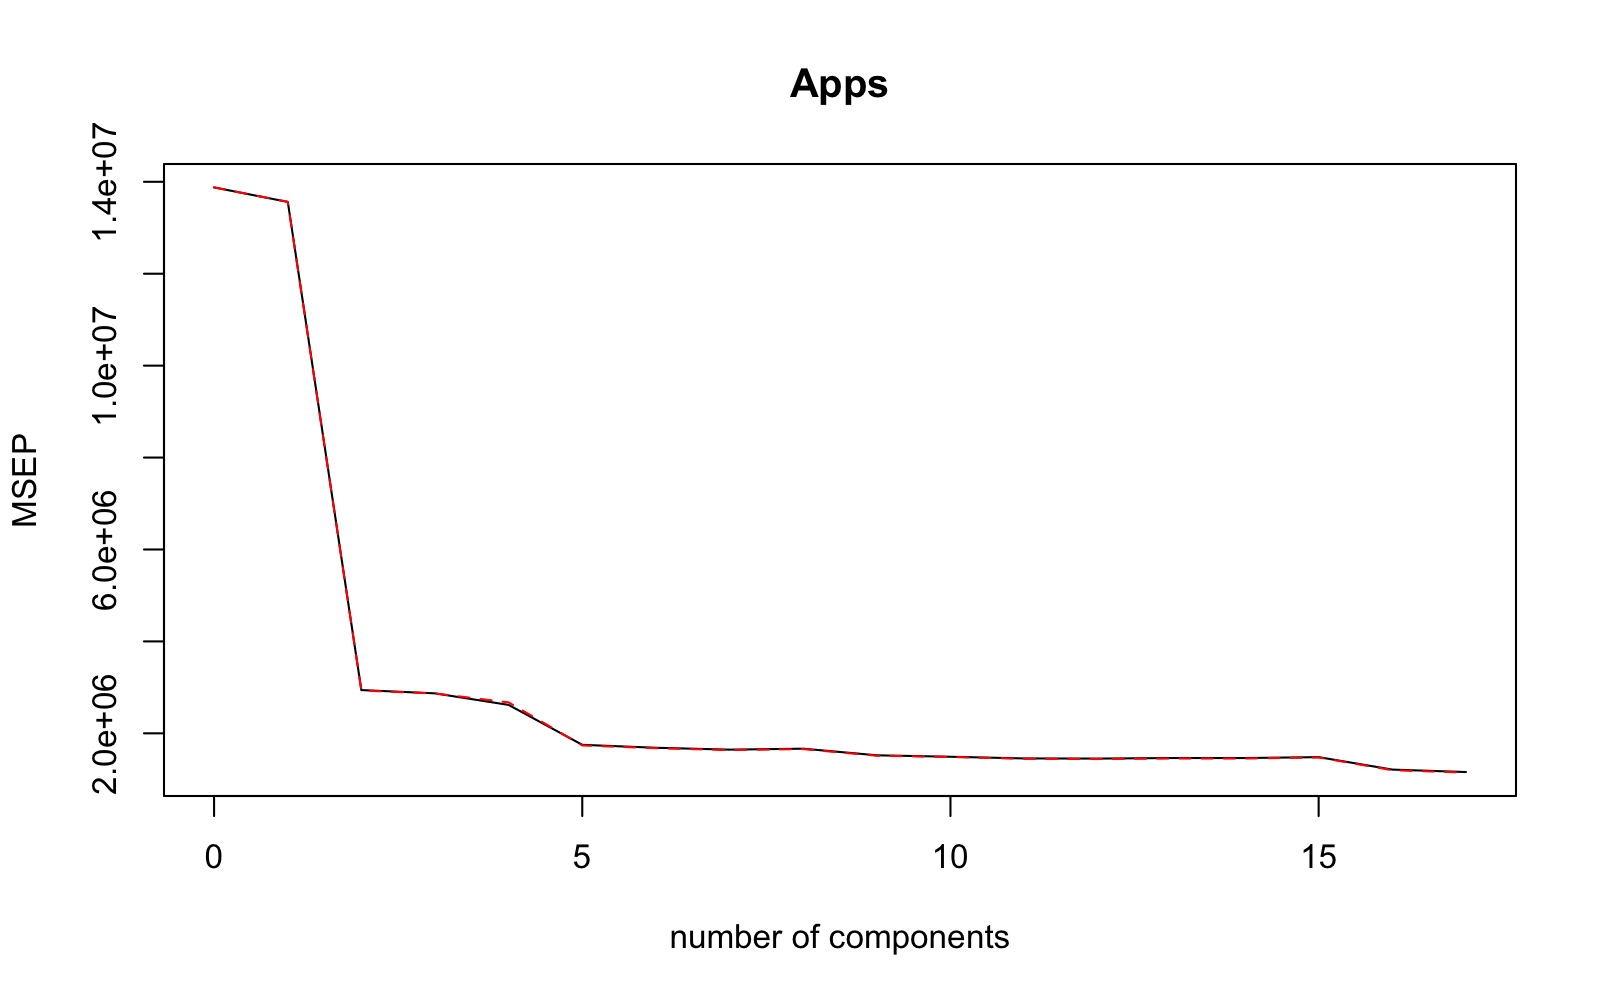
\includegraphics[width=0.8\textwidth]{MTH522_hw5_p2e.png}
	\end{center}
	\caption{.}
	\label{fig:MTH522_hw5_p2e}
\end{figure}

\newpage

\begin{program}
	\begin{verbatim}
	> pred.pcr = predict(fit.pcr, College.test, ncomp=10)
	> mean((College.test[, "Apps"] - data.frame(pred.pcr))^2)
	
	[1] 3014496
	\end{verbatim}
\end{program}
The test Residual sum of squares (RSS) for PCR 3014496  is higher than (b) 1538442.\\

(f) Fit a PLS model on the training set, with M chosen by cross-validation. Report the test error obtained, along with the value of M selected by cross-validation.\\

\begin{program}
	\begin{verbatim}
	> fit.pls = plsr(Apps~., data=College.train, scale=T, validation="CV")
	> validationplot(fit.pls, val.type = "MSEP")
	> dev.copy(png,"MTH522_hw5_p2f.png",width=8,height=4,units="in",res=200)
	>  dev.off()
	\end{verbatim}
\end{program}


\begin{figure}[htb]
	\begin{center}
		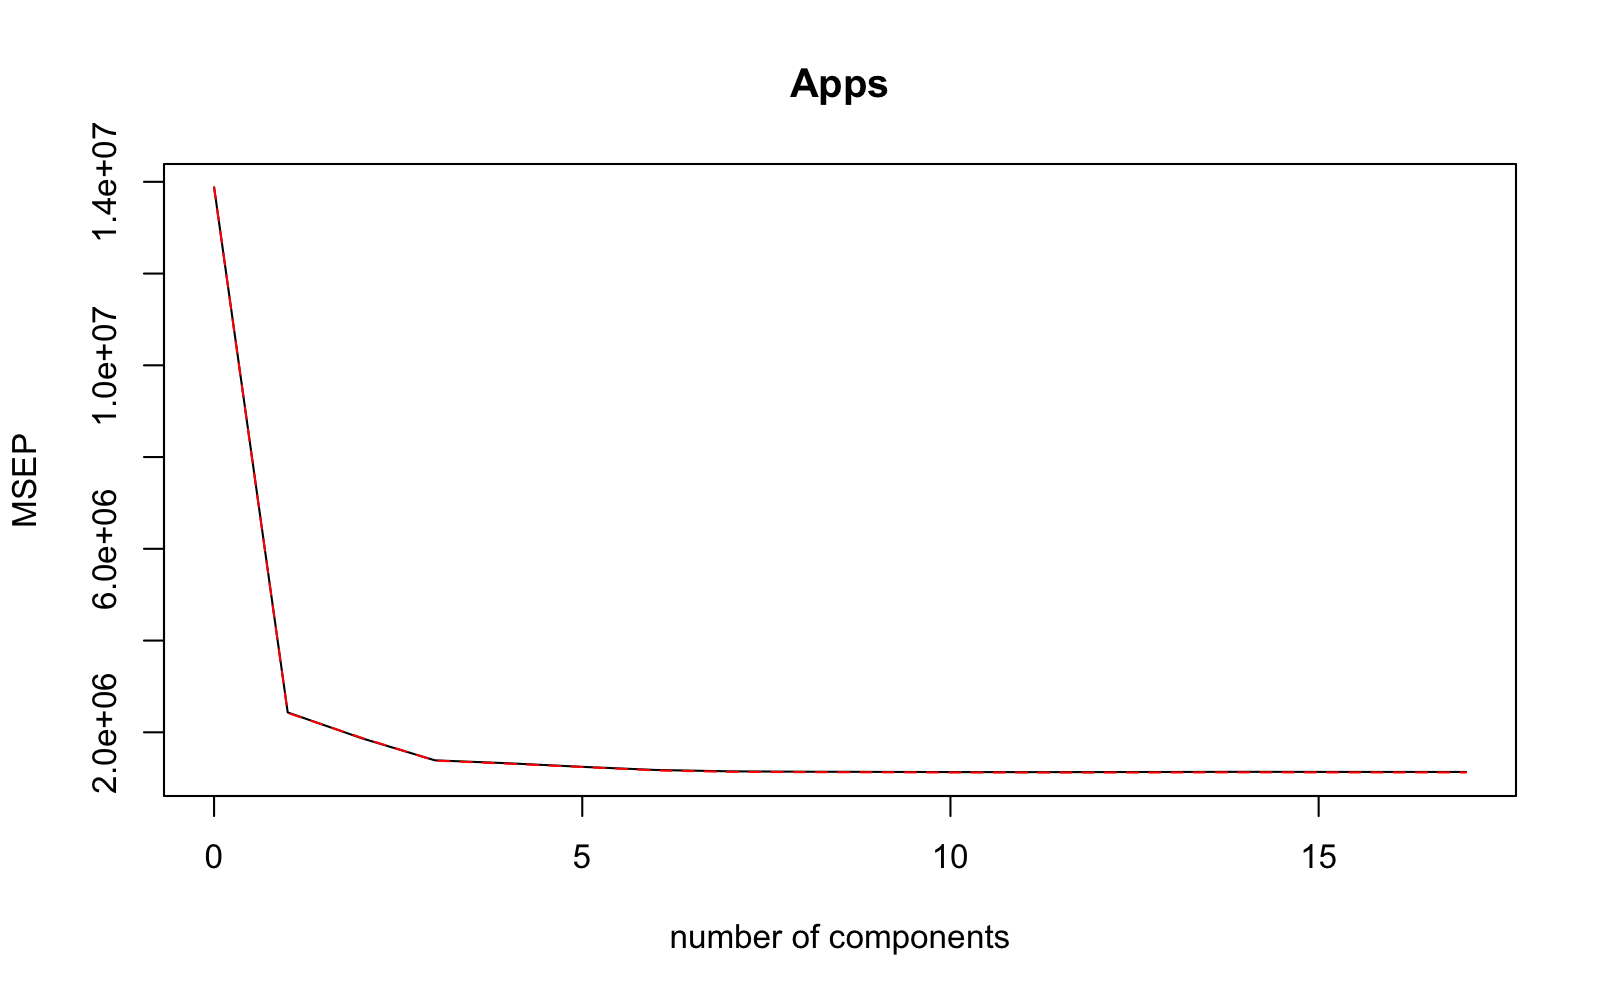
\includegraphics[width=0.8\textwidth]{MTH522_hw5_p2f.png}
	\end{center}
	\caption{.}
	\label{fig:MTH522_hw5_p2f}
\end{figure}

\begin{program}
	\begin{verbatim}
	> pred.pls <- predict(fit.pls, College.test, ncomp = 10)
	>  mean((pred.pls - College.test$Apps)^2)	
	[1] 1508987
	\end{verbatim}
\end{program}


\newpage

(g) Comment on the results obtained. How accurately can we predict the number of college applications received? Is there much difference among the test errors resulting from these five approaches?

Test $R^2$ for all five approaches;
\begin{program}
	\begin{verbatim}
	> test.avg = mean(College.test[, "Apps"])
	> lm.r2 = 1 - mean((College.test[, "Apps"] - pred.lm)^2)
	               /mean((College.test[, "Apps"] - test.avg)^2)
	> ridge.r2 = 1 - mean((College.test[, "Apps"] - pred.ridge)^2)
	            /mean((College.test[, "Apps"] - test.avg)^2)
	> lasso.r2 = 1 - mean((College.test[, "Apps"] - pred.lasso)^2)
	            /mean((College.test[, "Apps"] - test.avg)^2)
	> pcr.r2 = 1 - mean((College.test[, "Apps"] - data.frame(pred.pcr))^2) 
	             /mean((College.test[, "Apps"] - test.avg)^2)
	> pls.r2 = 1 - mean((College.test[, "Apps"] - data.frame(pred.pls))^2)
	            /mean((College.test[, "Apps"] - test.avg)^2)
	> barplot(c(lm.r2, ridge.r2, lasso.r2, pcr.r2, pls.r2), col="red", names.arg=c("OLS", 
	          "Ridge", "Lasso","PCR", "PLS"), main="Test R-squared")
	> dev.copy(png,"MTH522_hw5_p2g.png",width=8,height=6,units="in",res=200)
	>  	dev.off()
	\end{verbatim}
\end{program}


\begin{figure}[htb]
	\begin{center}
		
\includegraphics[width=0.8\textwidth]{MTH522_hw5_p2g.png}
	\end{center}
	\caption{.}
	\label{fig:MTH522_hw5_p2g}
\end{figure}

The barplot shows that test $R^2$ for OLS, Ridge Lasso are aound 0.9, PLS arround 0.93, but PCR has a smallest test number  arround 0.8. Foru models (not PCR) predict college application with high accuracy.



\newpage

{\bf Problem 3} (Chapter 6 Exercises 10):\\


We have seen that as the number of features used in a model increases, the training error will necessarily decrease, but the test error may not. We will now explore this in a simulated data set.\\

a) Generate a data set with p = 20 features, n = 1,000 observa- tions, and an associated quantitative response vector generated according to the model
\begin{equation} 
	Y =X\beta + \epsilon,	
\end{equation}

where $\beta$ has some elements that are exactly equal to zero.

\begin{program}
	\begin{verbatim}
	> p = 20
	> n = 1000
	> set.seed(1)
	> x = matrix(rnorm(n * p), n, p)
	> b = rnorm(p)
	> B[3] = 0
	> B[4] = 0
	> B[9] = 0
	> B[19] = 0
	> B[10] = 0
	> eps = rnorm(p)
	> y = x %*% b + eps
	\end{verbatim}
\end{program}

(b) Split your data set into a training set containing 100 observations and a test set containing 900 observations.

\begin{program}
	\begin{verbatim}
	> train = sample(seq(1000), 100, replace = FALSE)
	> x.train = x[train, ]
	> x.test = x[-train, ]
	> y.train = y[train, ]
	> y.test = y[-train, ]
		\end{verbatim}
\end{program}

\newpage


c) Perform best subset selection on the training set, and plot the training set MSE associated with the best model of each size.

\begin{program}
	\begin{verbatim}
	> install.packages("leaps")
	--- Please select a CRAN mirror for use in this session ---
	trying URL 'https://cran.cnr.berkeley.edu/bin/macosx/mavericks/contrib/3.3/leaps_2.9.tgz'
	Content type 'application/x-gzip' length 64598 bytes (63 KB)
	==================================================
	downloaded 63 KB


	The downloaded binary packages are in
	/var/folders/28/5cht8_x964n2w_4_wf_1tn3m0000gn/T//RtmpJKsxfo/downloaded_packages
	
	

	> library(leaps)
	> regfit.full = regsubsets(y ~ ., data = data.frame(x = x.train, y =
	+ y.train),
	+     nvmax = p)
	> val.errors = rep(NA, p)
	> x_cols = colnames(x, do.NULL = FALSE, prefix = "x.")
	> for (i in 1:p) {
	+     coefi = coef(regfit.full, id = i)
	+     pred = as.matrix(x.train[, x_cols %in% names(coefi)]) %*%
	+ coefi[names(coefi) %in%
	+         x_cols]
	+     val.errors[i] = mean((y.train - pred)^2)
	+ }
	> plot(val.errors, ylab = "Training MSE", pch = 19, type = "b")
	> dev.copy2pdf(file = "MTH522_hw5_p3c.pdf", width = 8, height = 4, out.type = "pdf")
	> dev.off()
	\end{verbatim}
\end{program}



\begin{figure}[htb]
	\begin{center}
		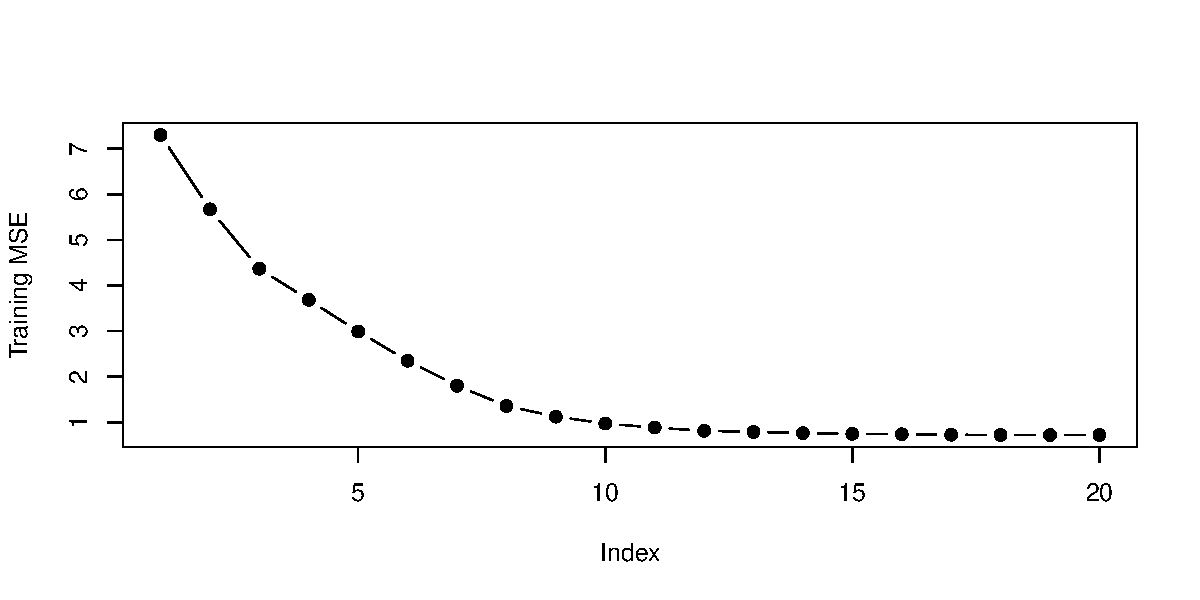
\includegraphics[width=0.8\textwidth]{MTH522_hw5_p3c.pdf}
	\end{center}
	\caption{.}
	\label{fig:MTH522_hw5_p3c}
\end{figure}

\newpage


(d) Plot the test set MSE associated with the best model of each size.


\begin{program}
	\begin{verbatim}
	> val.errors = rep(NA, p)
	> for (i in 1:p) {
	+     coefi = coef(regfit.full, id = i)
	+     pred = as.matrix(x.test[, x_cols %in% names(coefi)]) %*%
	+ coefi[names(coefi) %in%
	+         x_cols]
	+     val.errors[i] = mean((y.test - pred)^2)
	+ }
	> 

	> plot(val.errors, xlab = "Number of predictors", ylab = "Test MSE", pch = 19, type = "b")
	> dev.copy2pdf(file = "MTH522_hw5_p3d.pdf", width = 8, height = 5, out.type = "pdf")
	> dev.off()

	\end{verbatim}
\end{program}


\begin{figure}[htb]
	\begin{center}
		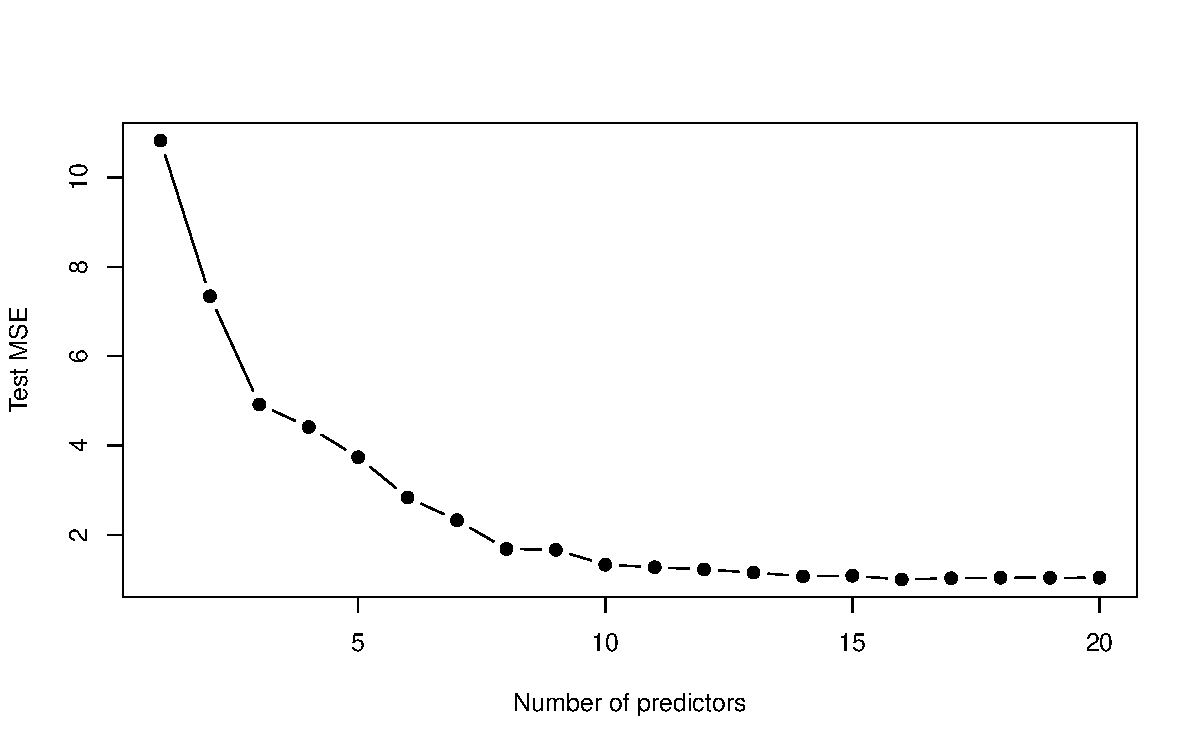
\includegraphics[width=0.8\textwidth]{MTH522_hw5_p3d.pdf}
	\end{center}
	\caption{.}
	\label{fig:MTH522_hw5_p3d}
\end{figure}




(e) For which model size does the test set MSE take on its minimum value? Comment on your results. If it takes on its minimum value for a model containing only an intercept or a model containing all of the features, then play around with the way that you are generating the data in (a) until you come up with a scenario in which the test set MSE is minimized for an intermediate model size.

\begin{program}
	\begin{verbatim}
	> which.min(val.errors)
	
	[1] 16
	\end{verbatim}
\end{program}
The 16 variables model has the smallest test MSE.

\newpage


(f) How does the model at which the test set MSE is minimized compare to the true model used to generate the data? Comment on the coefficient values.

\begin{program}
	\begin{verbatim}
	> coef(regfit.full, which.min(val.errors))
	(Intercept)        x.1         x.2         x.5         x.6         x.7         x.8 
	0.09613244  0.28256751  0.19385802  0.99994674 -0.28597795 -1.50482273  0.77817125 
 	    x.11        x.12        x.13        x.14        x.15        x.16        x.17 
	0.90815918  0.48477881 -0.19747066 -0.71978955 -0.74282068 -0.33900837  0.12234642 
	      x.18        x.19        x.20 
	1.74270174 -0.12435131 -1.03003019 	
	\end{verbatim}
\end{program}
The best model caught all but one zeroed out coefficient at x.19.

(g) How does this compare to the test MSE plot from (d)?

\begin{program}
	\begin{verbatim}
	> val.errors = rep(NA, p)
	> for (i in 1:p) {
	+     coefi = coef(regfit.full, id = i)
	+     val.errors[i] = sqrt(sum((B[x_cols %in% names(coefi)] -
	+ coefi[names(coefi) %in% x_cols])^2) +
	+         sum(B[!(x_cols %in% names(coefi))])^2)
	+ }
	> plot(val.errors, xlab = "number of coefficients", ylab = "error
	+ between estimated and true coefficients")
	
	> dev.copy2pdf(file = "MTH522_hw5_p3g.pdf", width = 8, height = 4, out.type = "pdf")
	>  dev.off()	
   	\end{verbatim}
\end{program}

\begin{figure}[htb]
	\begin{center}
		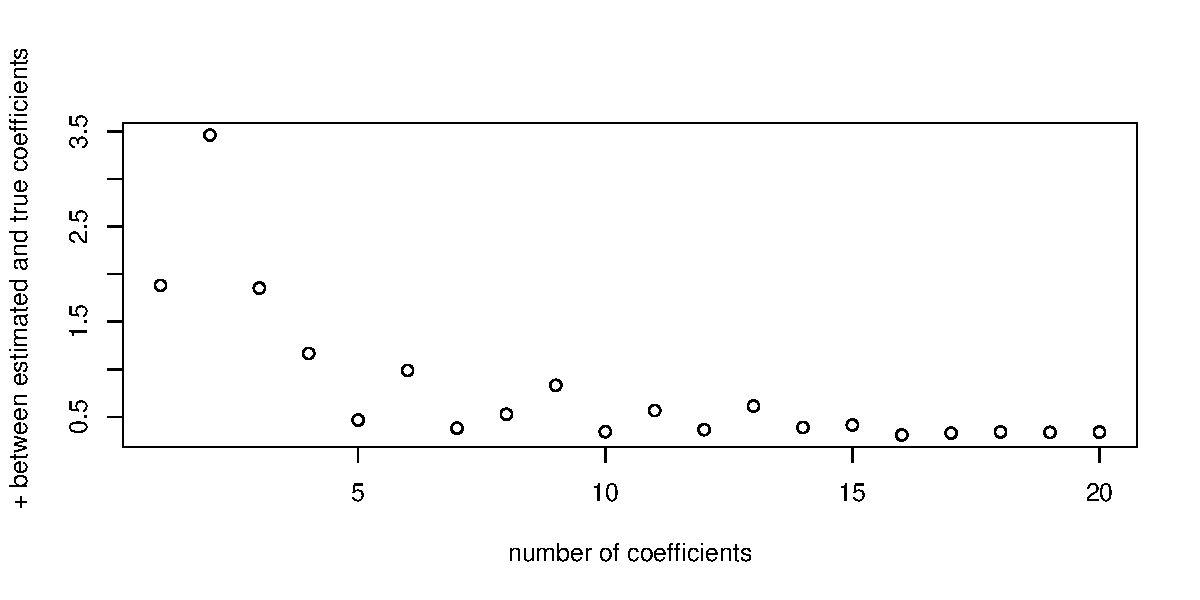
\includegraphics[width=0.8\textwidth]{MTH522_hw5_p3g.pdf}
	\end{center}
	\caption{.}
	\label{fig:MTH522_hw5_p3g}
\end{figure}


\newpage





\begin{program}
	\begin{verbatim}
	> which.min(val.errors)

	[1] 16
	\end{verbatim}
\end{program}

Teset error is minimized with 16 parameter model. So, a better fit of true coefficients doesn't necessarily mean a lower test MSE.\\
\\
\\
{\bf Problem 4} (Chapter 6 Exercises 11):\\
We will now try to predict per capita crime rate in the Boston data set.
(a) Try out some of the regression methods explored in this chapter, such as best subset selection, the lasso, ridge regression, and PCR. Present and discuss results for the approaches that you consider.

\begin{program}
	\begin{verbatim}
	> set.seed(1)
	> library(MASS)
	
	Attaching package: ‘MASS’
	
	The following object is masked _by_ ‘.GlobalEnv’:
	
	Boston
	
	
	> library(leaps)
	> library(glmnet)
	Loading required package: Matrix
	Loading required package: foreach
	foreach: simple, scalable parallel programming from Revolution Analytics
	Use Revolution R for scalability, fault tolerance and more.
	http://www.revolutionanalytics.com
	Loaded glmnet 2.0-5
	\end{verbatim}
\end{program}


{\bf Best Subset Selection Method}


\begin{program}
	\begin{verbatim}
	> k = 10
	> p = ncol(Boston) - 1
	> folds = sample(rep(1:k, length = nrow(Boston)))
	> cv.errors = matrix(NA, k, p)
	> for (i in 1:k) {
	     best.fit = regsubsets(crim ~ ., data = Boston[folds != i, ], nvmax = p)
	     for (j in 1:p) {
	         pred = predict(best.fit, Boston[folds == i, ], id = j)
	         cv.errors[i, j] = mean((Boston$crim[folds == i] - pred)^2)
	 } }
	> rmse.cv = sqrt(apply(cv.errors, 2, mean))
	> plot(rmse.cv, pch = 19, type = "b")
	>  dev.copy2pdf(file = "MTH522_hw5_p4a.pdf", width = 8, height = 6, out.type = "pdf")
	>  dev.off()
	
	
	
	\end{verbatim}
\end{program}

\begin{figure}[htb]
	\begin{center}
		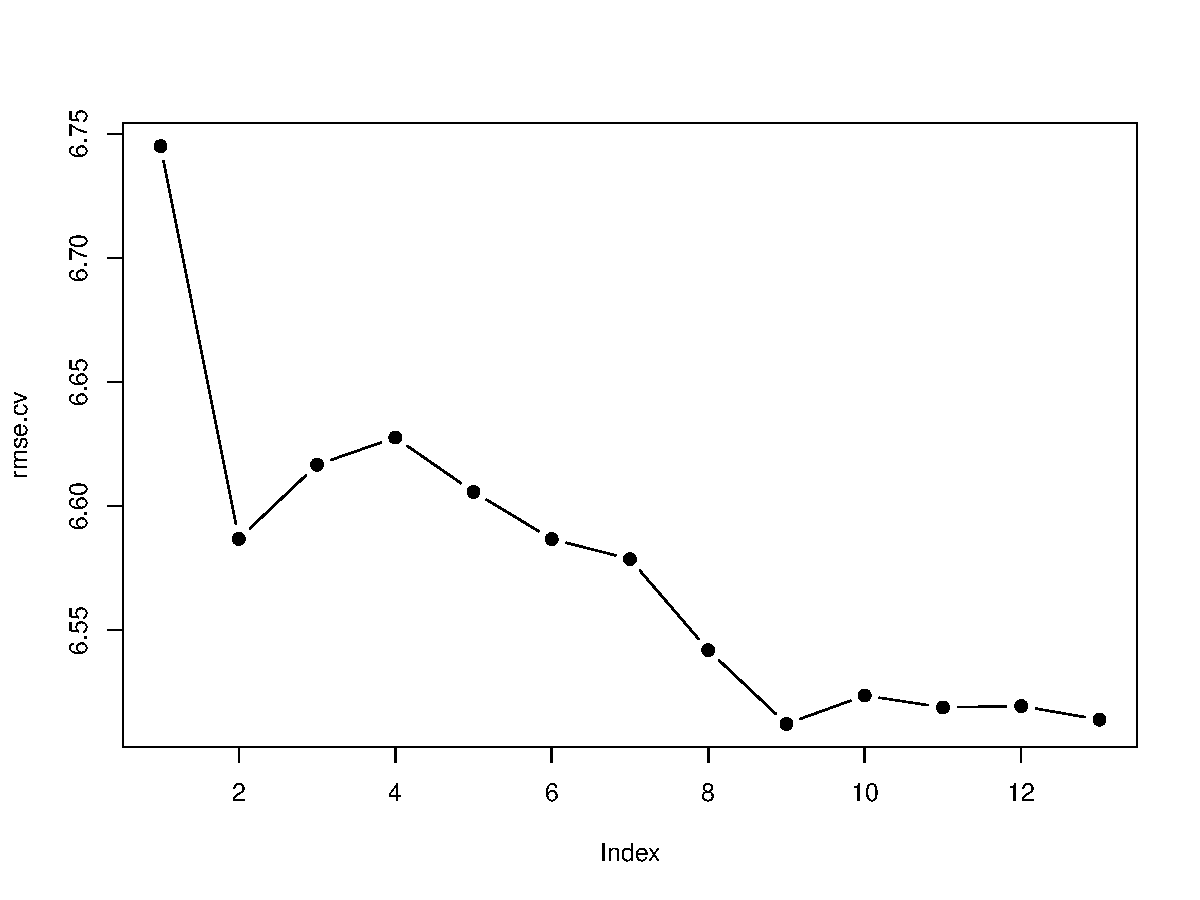
\includegraphics[width=0.8\textwidth]{MTH522_hw5_p4a.pdf}
	\end{center}
	\caption{.}
	\label{fig:MTH522_hw5_p4a}
\end{figure}


\begin{program}
	\begin{verbatim}
	> which.min(rmse.cv)

	[1] 9
	
	
	> rmse.cv[which.min(rmse.cv)]

	[1] 6.512237
	\end{verbatim}
\end{program}

\newpage


{\bf Lasso}

\begin{program}
	\begin{verbatim}
	> x = model.matrix(crim ~ ., Boston)[, -1]
	>  y =  Boston$crim
	>  cv.lasso = cv.glmnet(x, y, type.measure = "mse")
	>  plot(cv.lasso)
	>  dev.copy2pdf(file = "MTH522_hw5_p4a_lasso.pdf", width = 8, height = 6, out.type = "pdf")
	>   dev.off()
	\end{verbatim}
\end{program}

\newpage

\begin{figure}[htb]
	\begin{center}
		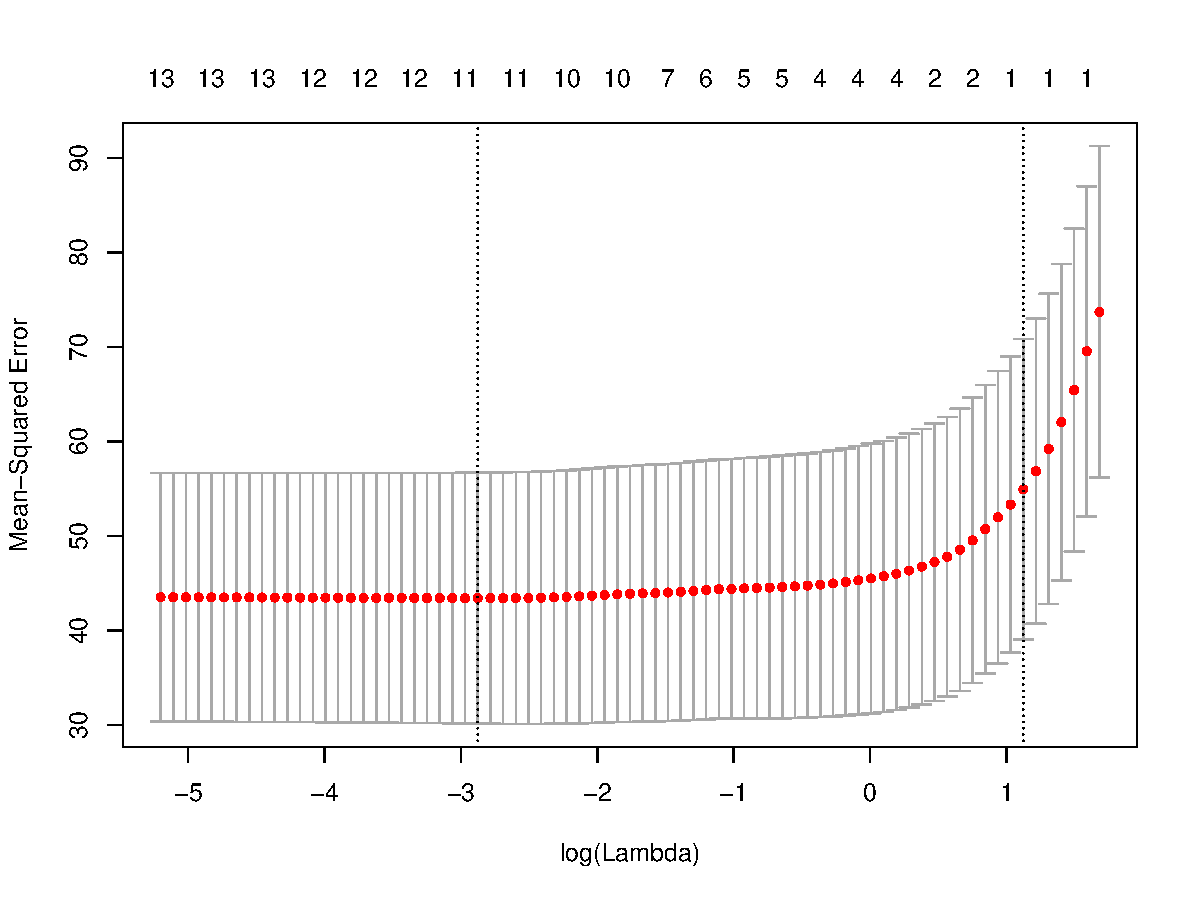
\includegraphics[width=0.8\textwidth]{MTH522_hw5_p4a_lasso.pdf}
	\end{center}
	\caption{.}
	\label{fig:MTH522_hw5_p4a_lasso}
\end{figure}


\begin{program}
	\begin{verbatim}
	> coef(cv.lasso)
	14 x 1 sparse Matrix of class "dgCMatrix"
	1
	(Intercept) 1.0894283
	zn          .        
	indus       .        
	chas        .        
	nox         .        
	rm          .        
	age         .        
	dis         .        
	rad         0.2643196
	tax         .        
	ptratio     .        
	black       .        
	lstat       .        
	medv        .        	

	> sqrt(cv.lasso$cvm[cv.lasso$lambda == cv.lasso$lambda.1se])

	[1] 7.411171
	\end{verbatim}
\end{program}





\newpage
{\bf Ridge Regression}

\begin{program}
	\begin{verbatim}
	> x = model.matrix(crim ~ . - 1, data = Boston)
	> y =  Boston$crim
	> cv.ridge = cv.glmnet(x, y, alpha = 0 , type.measure = "mse")
	> plot(cv.ridge)
	> dev.copy2pdf(file = "MTH522_hw5_p4a_ridge.pdf", width = 8, height = 6, out.type = "pdf")  
	>   dev.off()
	\end{verbatim}
\end{program}

\begin{figure}[htb]
	\begin{center}
		\includegraphics[width=0.8\textwidth]{MTH522_hw5_p4a_ridge.pdf}
	\end{center}
	\caption{.}
	\label{fig:MTH522_hw5_p4a_ridge}
\end{figure}

\newpage

\begin{program}
	\begin{verbatim}
	> coef(cv.ridge)
	14 x 1 sparse Matrix of class "dgCMatrix"
	1
	(Intercept)  1.984601820
	zn          -0.002712896
	indus        0.023751842
	chas        -0.120843958
	nox          1.499819910
	rm          -0.118580408
	age          0.005022922
	dis         -0.075115440
	rad          0.034570984
	tax          0.001596306
	ptratio      0.056535699
	black       -0.001981669
	lstat        0.027880296
	medv        -0.018358122
	
	
	> sqrt(cv.ridge$cvm[cv.ridge$lambda == cv.ridge$lambda.1se])
	
	[1] 7.848479
	\end{verbatim}
\end{program}




\newpage

{\bf PCR}

\begin{program}
	\begin{verbatim}
	> library(pls)
	
	Attaching package: ‘pls’
	
	The following object is masked from ‘package:stats’:
	
	loadings
	
	> pcr.fit = pcr(crim ~ ., data = Boston, scale = TRUE, validation = "CV")
	> summary(pcr.fit)
	
	Data: 	X dimension: 506 13 
	Y dimension: 506 1
	Fit method: svdpc
	Number of components considered: 13
	
	VALIDATION: RMSEP
	Cross-validated using 10 random segments.
	(Intercept)  1 comps  2 comps  3 comps  4 comps  5 comps  6 comps
	CV            8.61    7.177    7.179    6.735    6.716    6.730    6.736
	adjCV         8.61    7.175    7.177    6.732    6.712    6.727    6.732
	7 comps  8 comps  9 comps  10 comps  11 comps  12 comps  13 comps
	CV       6.726    6.598    6.599     6.590     6.571     6.557     6.491
	adjCV    6.722    6.594    6.595     6.585     6.566     6.550     6.484
	
	TRAINING: % variance explained
	1 comps  2 comps  3 comps  4 comps  5 comps  6 comps  7 comps
	X       47.70    60.36    69.67    76.45    82.99    88.00    91.14
	crim    30.69    30.87    39.27    39.61    39.61    39.86    40.14
	8 comps  9 comps  10 comps  11 comps  12 comps  13 comps
	X       93.45    95.40     97.04     98.46     99.52     100.0
	crim    42.47    42.55     42.78     43.04     44.13      45.4	
	\end{verbatim}
\end{program}

13 component pcr fit has lowest 6.491(CV) and  6.484 (adjCV) RMSEP.\\






(b) Propose a model (or set of models) that seem to perform well on this data set, and justify your answer. Make sure that you are evaluating model performance using validation set error, cross-validation, or some other reasonable alternative, as opposed to using training error.\\

As we can see above the model with cross-validate error is the one chosen by the Best Subset Selection Method.\\


(c) Does your chosen model involve all of the features in the data set? Why or why not?\\

No, it does not involve all of the features in the data set. The best subset selection method has only 13 component.



\end{document}





